% !Mode:: "TeX:UTF-8"
%% 请使用 XeLaTeX 编译本文.
% \documentclass{WHUBachelor}% 选项 forprint: 交付打印时添加, 避免彩色链接字迹打印偏淡. 即使用下一行:
\documentclass[forprint]{WHUBachelor}

\begin{document}
\renewcommand{\thelstlisting}{\arabic{section}.\arabic{lstlisting}}
%%%%%%% 下面的内容, 据实填空.

\miji{ }                                      % 密级. 没有就空着.
\StudentNumber{201731062232} % 填写自己的学号

\title{三维空间最短路径算法设计与实现}
\Etitle{Design and Implementation of Shortest Path Algorithm in Three-Dimensional Space} % 英文题目
\author{陈东} % 作者名字
\Eauthor{Chen dong}            %作者英文名
\Csupervisor{刘小玲\quad 讲师}        %指导教师中文名、职称
\Esupervisor{Liu Xiao Ling} %指导教师英文名、职称
\Grade{2017}
\Cmajor{软件工程}                  % 专业中文名
\Emajor{Software Engineering}% 专业英文名
\Cschoolname{计算机科学学院}          % 学院名
\Eschoolname{School of Computer Science} %学院英文名. 不确定的话, 请看一下自己学院的网页上是怎么写的. 别搞错了!
\date{二〇二一年五月}                    % 日期, 要注意和英文日期一致!!
\Edate{May, 2021}                       % 英文封面日期

%-----------------------------------------------------------------------------
\pdfbookmark[0]{封面}{title}         % 封面页加到 pdf 书签
\maketitle
\frontmatter
\pagenumbering{Roman}              % 正文之前的页码用大写罗马字母编号.
%-----------------------------------------------------------------------------
% !Mode:: "TeX:UTF-8"

%%% 此部分需要自行填写: (1) 中文摘要及关键词 (2) 英文摘要及关键词
%%%%%%%%%%%%%%%%%%%%%%%%%%%%%
%%% -------------  英文封面 (无需改动)-------------   %%%
%%%%%%%%%%%%%%%%%%%%%%%%%%%%%
\thispagestyle{empty}
\renewcommand{\baselinestretch}{1.5}  %下文的行距
\vspace*{0.5cm}
\begin{center}
{\Large \bf BACHELOR'S DEGREE THESIS \\[1ex] OF WUHAN UNIVERSITY }
\end{center}
\vspace{2.5cm}
\begin{center}{\zihao{2} \the\Etitle \par}\end{center}

\vfill

\begin{center}
\zihao{4}
\begin{tabular}{ r l }
 School (Department): & {\sc \the\Eschoolname}\\
  Major:          &   {\sc\the\Emajor}  \\
 Candidate:      &  {\sc \the\Eauthor}      \\
 Supervisor:     &  {\sc \the\Esupervisor}
\end{tabular}

\vspace*{2cm}
\begin{center}
   \ifprint % 文档打印, 使用黑白校徽.
  
\includegraphics[height=4cm]{whu.eps}       %%  黑白的.
  \else
  
\includegraphics[height=4cm]{whulogo.eps} %%  彩色的.
  \fi
\end{center}


\zihao{-2}
%\the\Schoolname\\
{\sc Wuhan University}

\vspace*{1.0cm}

\the\Edate

\end{center}
%%% 郑重声明部分无需改动

%%%---- 郑重声明 (无需改动)------------------------------------%
\newpage
\vspace*{20pt}
\begin{center}{\ziju{0.8}\textbf{\songti\zihao{2} 郑重声明}}\end{center}
\par\vspace*{30pt}
\renewcommand{\baselinestretch}{2}

{\zihao{4}%

本人呈交的学位论文, 是在导师的指导下, 独立进行研究工作所取得的成果,
所有数据、图片资料真实可靠. 尽我所知, 除文中已经注明引用的内容外,
本学位论文的研究成果不包含他人享有著作权的内容.
对本论文所涉及的研究工作做出贡献的其他个人和集体,
均已在文中以明确的方式标明. 本学位论文的知识产权归属于培养单位.\\[2cm]

\hspace*{1cm}本人签名: $\underline{\hspace{3.5cm}}$
\hspace{2cm}日期: $\underline{\hspace{3.5cm}}$\hfill\par}
%------------------------------------------------------------------------------
\baselineskip=23pt  % 正文行距为 23 磅
%------------------------------------------------------------------------------





%%======中文摘要===========================%
\begin{cnabstract}
本文主要介绍和讨论了武汉大学本科毕业论文的~\LaTeX~模板.
指明了编译方法, 强调了公式排版的一些细节问题, 也指出了一些常见的排版错误.



\end{cnabstract}
\par
\vspace*{2em}


%%%%--  关键词 -----------------------------------------%%%%%%%%
%%%%-- 注意: 每个关键词之间用“;”分开,最后一个关键词不打标点符号
\cnkeywords{毕业论文; \LaTeX{}; 模板;  }


%%====英文摘要==========================%


\begin{enabstract}
This thesis is a study on the theory of \dots.

\end{enabstract}
\par
\vspace*{2em}

%%%%%-- Key words --------------------------------------%%%%%%%
%%%%-- 注意: 每个关键词之间用“;”分开,最后一个关键词不打标点符号
 \enkeywords{\LaTeX{};  }
    % 加入摘要, 申明.
%==========================把目录加入到书签==============================%%%%%%
%\pdfbookmark[0]{目录}{toc}
\tableofcontents
\mainmatter %% 以下是正文
%%%%%%%%%%%%%%%%%%%%%%%%%%%--------main matter-------%%%%%%%%%%%%%%%%%%%%%%%%%%%%%%%%%%%%

\chapter{绪论}
 
 \section{论文研究背景与意义}
\subsection{选题的背景}
对于许多实际生活中需要求得两个地方之间的路径和距离,并且考虑障碍物的影响,以提供后续决策等的帮助,例如房间当中两个窗户之间风的流向轨迹,在山体之间修路等问题的求解时需要计算出起点到终点之间的最短路径。对于小数据范围如房屋空间,不需要复杂的数学模型建模转换为二维模型以求解最短路径,可以在考虑一定误差范围内将障碍物转换为AABB包围盒,利用最短路径算法直接在三维空间中求解起点到终点的近似最短路径。
\subsection{选题的技术现状}
本算法通过将空间离散为若干个格子点,将障碍物近似为每一边都平行于一个坐标平面的简单六面体,通过常规最短路径算法:BFS广度优先搜索算法和A*寻路算法求解给定起点到终点不经过障碍物的的可行路径,再拟合成若干线段,通过检查线段是否穿过障碍物实现路径拟合,最后通过动态规划计算最优路径长度。
\subsection{选题的意义}
完成本选题,是为了设计并实现算法以解决实际项目中遇到的路径长度求解问题,提供近似最短路径和欧式距离以提供路径选择参考。
\section{国内外研究现状}
国内外对于三维最短路径算法的研究一般基于数字高程模型(Digital Elevation Model,简称DEM),是通过用一组有序数值阵列形式表示地面高程的数据集。对于DEM给出的地面高程信息,在测绘、水文、气象等应用地面模型的领域都取得了突破性进展。本文不利用DEM模型,而是将三维空间离散为若干个格点,再应用最短路径算法在格点间,求得起点格点到终点格点的最短路径后再将格点之间的路线拟合为线段的实现方式。
\section{论文组织结构}
本文针对三维空间路径规划问题开展研究,首先将障碍物的aabb包围盒以某个尺度离散为具体的格点,对格点进行不可访问标记处理;随后基于所给的起点,采用最短路径算法求得到终点所经过的格点序列,提出一种基SPFA和A*的最短路径算法实现,同时对比了基于不同最短路径算法之间的空间-时间开销。本文的组织结构如下:\\第一章:本章主要介绍研究课题的背景和意义,三维空间最短路径研究现状及发展的趋势,并讨论了国内外在相关方面的研究状况及其应用前景,给出本文的主要贡献、创新性和组织结构。\\第二章:本章主要介绍了最短路径模型、二维和三维空间最短路径的区别和联系、图的概念、存储方式并对比了不同存储方式的优缺点。最后,总结和阐述了三维空间最短路径的规划方法。\\第三章:本章主要对三维空间最短路径求解算法进行分类总结,提出将三维空间离散为格点后,在格点图上进行BFS、A*、SPFA等算法求解最短路径的效率和开销。\\第四章:对全文进行了总结,对未来基于三维空间的最短路径算法深入研究作出了展望。 %chapter1

\setcounter{table}{0}
\setcounter{figure}{0}
\section{最短路径优化算法研究综述}

\subsection{图}
\par 图论,是组合数学分支,和其他数学分支也有密切关系,如群论、拓扑学。图是图论的主要研究对象,图是给点若干顶点以及两顶点所构成的图形,这种图形可以用来描述事物之间的某种特定关系。
顶点可以用来描述某种事物,连接两顶点可以代表事物之间存在的某种关系,如顶点代表学习任务,连接顶点代表学习该任务之前需要学习的其他任务。图论起源于著名的柯尼斯堡七桥问题即著名的欧拉图一笔画问题。该问题于1736年被欧拉解决,因此普遍认为欧拉是图论的创始人\upcite{Graphtheory}。通常在图论中,以有序对$G=(V,E)$,其中V是点集;$E\subset \{\{x, y\}:(x,y)\in V^2,x\ne y\}$是边集,由所有顶点序列构成,其中一条边$\{x,y\}$中的x,y被称作边的端点;
图的分类分为有向图和无向图,其中有向图是指给图的每条边都规定一个方向,其边称为有向边,以$<x,y>$;相反,边没有方向的图称为无向图,无向边以$(x,y)$表示,则在边集会同时存在$(x,y),(y,x)$。并且V,E的元素个数通常都是有限的,图的阶数是其顶点个数$|V|$,图的边数是$|E|$。每条边都连接两个不同的顶点且没有两条不同的边连接一对相同顶点的图称为\textbf{简单图},可能有\textbf{多重边}连接同一对顶点的图成为\textbf{多重图}。其中最短路径问题、最小生成树问题、关键路径问题都属于是基于图上的问题,并提出了相应的解决方案。如图\ref{fig:graph_ex}分别是无向图和有向图的一个实例。其中,对于实际问题中每条边代表了从顶点$x$到$y$所需要的权值的图叫做带权图,其中边上的权值也叫边的长度。
\begin{figure}[!htb]
  \centering
  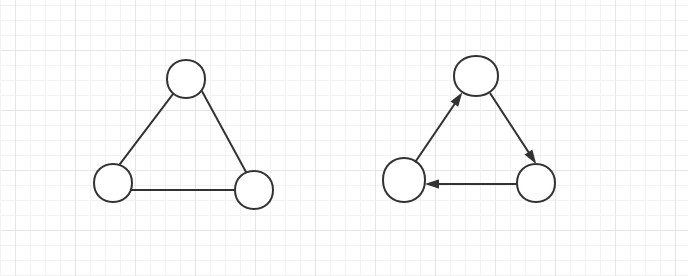
\includegraphics[width=10cm]{figures/graph_ex.png}
  \caption{无向图和有向图实例}  
  \label{fig:graph_ex}
\end{figure}
\par\textbf{三维空间}是类似我们生存的空间的数学模型,由长、宽、高三个维度,也即是三维欧几里得空间,定义欧几里得平面为装备了内积的二维实数的向量空间。满足
\begin{enumerate}[.]
    \item 在这个向量空间中的向量对应欧几里得平面中的点,
    \item 在向量空间中的加法运算对应于平移,
    \item 内积蕴含了角和距离的概念,它可被用来定义旋转。
\end{enumerate}\par
如图\ref{fig:3axis}就是三维欧几里得空间的示意图,三个轴相互垂直,点的坐标为其到三个轴的投影。
\begin{figure}[!htb]
  \centering
  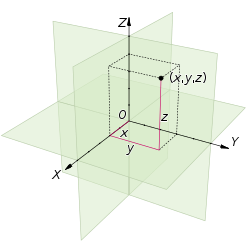
\includegraphics[width=8cm]{figures/3axis.png}
  \caption{三维欧几里得空间}  
  \label{fig:3axis}
\end{figure}
\par 一般在计算机中存储图信息,有以下几种方式
\begin{enumerate}
    \item 邻接矩阵,使用多维数组记录点与点之间的边权信息;
    \item 邻接表,使用链表等数据结构维护该点到其他点的边信息;
    \item 十字链表,将有向图的邻接表和逆邻接表的结合;
    \item 邻接多重表,将无向图的邻接表和逆邻接表的结合;
\end{enumerate}\par
邻接矩阵是应用多维数组保存的点和点之间的关系,因此可以很容易的判断两个点之间的关系,但缺点在于占用空间大,尤其对于多维空间时保存信息时需要占用大量的存储空间;邻接表使用链表保存点所连接的边信息,节省了空间,但不易得到两点之间的关系;十字链表和邻接多重表都能节省空间、快速判断点与点之间的关系,但缺点是实现起来比较复杂。

\subsection{最短路径规划}
\par 首先,在图中的\textbf{路径}是指从顶点$u$到顶点$v$的一个序列$v_0,e_1,v_1,e_2,v_2,\dots,e_k,v_k$,有时简写为$v_0\rightarrow v_1\rightarrow v_2\rightarrow\dots\rightarrow v_k$,其中$e_i$表示起点终点为$v_{i-1}$及$v_i$;$k$称为路径的长度,即经过的边的数量;$v_0=u$称为路径的起点;$v_k=v$称为路径的终点。当没有必要区分多重边时,就用顶点序列$x_0,x_1,\dots, x_n$表示通路$e_1,e_2,\dots,e_n$,其中对于$i=1,2,\dots,n,f(e_i)={x_{i-1}, x_i}$,这种记法仅仅指出通路所经过的顶点。其中论文求解的最短路径是指:若从顶点$u$到顶点$v$之间长度最短的路径,即是加权图中一条路径的长度是这条路径上各条边的总和最小。
最短路径问题是图论研究的一个经典算法问题,目的在于求出两顶点之间的最短路径。算法具体的形式有
\begin{itemize}
    \item 确定起点的最短路径问题,也即已知起始起点求最短路径的单源最短路径问题;
    \item 确定终点的最短路径问题,与确定起点的问题相反,该问题是已知终结顶点,求最短路径的问题;
    \item 确定起点终点的最短路问题,即已知起点和终点,求两顶点之间的最短路径;
    \item 全局最短路径问题,也叫多源最短路问题,求出图中所有的最短路径。
\end{itemize}
\par 用于解决最短路径问题的算法叫做“最短路径算法”,常用的路径算法有:
\begin{itemize}
    \item BFS算法;
    \item Dijkstra算法;
    \item A*算法;
    \item Bellman-Ford算法;
    \item SPFA算法(Bellman-Ford算法的改进版本);
    \item Floyd算法;
\end{itemize}
\par 广度优先搜索(BFS)和深度优先搜索(DFS)会从起点开始求解出可行路径,但由于DFS需要求解所有路径才知道最短路径,而BFS算法的特点是逐层扩展的,决定了其不需要遍历所有的路径就能找到最短路径。Dijkstra、A*、Bellman-Ford、SPFA算法都是用于解决单源最短路径,其中Dijskra用于正权路径最短路径求解,Bellman-Ford、SPFA、A*可用于正负权路径最短路径求解,Floyd用于解决多源最短路径;其中不同算法在基于不同的图结构上拥有不同的时间、空间复杂度,其中Dijkstra和A*在寻路算法中应用广泛,由于A*使用了估值函数,会更倾向的选择路线,更加节省内存空间。
\subsection{本章小结}
\par{\kaishu 本章主要介绍了图结构的定义以及常见的计算机存储图结构的数据结构,以及介绍了路径定义和最短路径的定义和求解算法。对于常见的图结构,使用邻接矩阵和邻接表在不同的应用领域都有很好的发挥,如邻接矩阵可以很快的得到顶点与顶点之间的关系,但需要记录每个顶点到其他所有顶点的关系,占用的内存空间较大;邻接表使用链表结构存储每个顶点所连接的边信息,可以节省大量的空间,但不容易得到顶点与顶点的关系。随后介绍了关于对图上最短路径求解的常用算法,如单源最短路径算法,有用于正权图最短路径求解的Dijskra算法,正负权都适用的Bellman-Ford、SPFA算法,基于估值函数优化的A*算法在寻路方面有广泛的应用;以及用于多源最短路径求解的Floyd算法。} %chapter2

\chapter{最短路径算法实现}
\section{最短路径算法分析}
\par 在二维空间中,通常是基于二维垂直的欧几里得空间,其中x轴和y轴垂直,顶点通常以类似经纬度形式给出,如~(x,y)~代表该顶点分别该点坐标分别在x轴、y轴上的长度分量,点~(a,b)~在~x~轴的分量为~a~,在~y~轴的分量为~b~;其中顶点之间会与若干条路径相连,其中路径不能经过相关障碍物,路径的权值可以是该条路径的长度或该条路径所需费用,记为~W(i,j)~表示第~i~个顶点到第~j~个顶点的边的权值。例如在运输网络中,顶点代表的是不同城市的集散地,顶点之间的路径就是城市之间的交通网,路径的权值代表该条交通路线所需要的时间,则所求的顶点到顶点的最短路径即是最短时间的路线。

\subsection{基于Dijkstra算法的最短路径求解}
\par Dijkstra该算法基于贪心的思想,解决了图~G=<V,E>~上带权的单源最短路径问题,通过设置一顶点集合~S~,在集合S中所有的顶点与源点s之间的最终最短路径权值均已被计算出来。算法反复选择最短路径估计最小的点$u\in V-S$并将~u~加入到~S~中,最终计算出源点到其他所有点的最短距离。举例来说,若图中的顶点代表城市,而边上的权值表示城市间开车行车的距离,该算法可以用来找到两个城市之间的最短路径。但是Dijkstra算法并不能有效处理带有负权边的图。
\par 算法描述:Dijkstra算法通过保留目前为止所找到的每个顶点$v\in V$从~s~到~v~的最短路径来工作。初始时,原点s的路径权重被赋为0。同时把所有顶点的路径长度设为无穷大,即表示我们不知道任何通向这些顶点的路径。当算法结束后,~d[v]~中存储的便是从s到v的最短路径,或者如果路径不存在的话是无穷大。
\par 松弛操作是Dijkstra的基础操作:如果存在一条从u到v的边,那么从s到v的一条新路径是将边$w(u,v)\in E$添加到从s到u的路径尾部来拓展一条从s到v的路径。这条路径的长度是$d[u]+w(u,v)$。若这个值比目前已知的$d[v]$的值要小,那么可以用这个值来替代当前$d[v]$中的值。松弛边的操作一直运行到所有的$d[v]$都代表从s到v的最短路径的长度值。由于基于松弛操作,因此若存在负权值边中的负环时会重复松弛,导致无法正确求解出最短路径。
\par 算法维护两个顶点集合openList和clostList,集合openList保留所有已知实际最短路径值的顶点,而集合clostList则保留其他所有顶点。集合S初始状态为空,而后每一步都有一个顶点从Q移动到S。这个被选择的顶点是Q中拥有最小的$d[u]$值的顶点。当一个顶点~u~从~Q~中转移到了~S~中,算法对u的每条外接边$w(u,v)$进行松弛。
\par 算法的步骤如下
\begin{enumerate}
    \item 输入边全为正权的图,G中带有顶点V=$v_0,v_1,v_2\dots$和若干边$w(v_i,v_j)$
    \item 设置一个待检测列表clostList和一个不需检测列表clostList;
    \item 将起始点startPoint加入openList中;
    \item 初始化距离向量~d~,其中startPoint的距离为0,其他全为正无穷;
    \item 检测openList,找出~d~值最小的一个点,将此节点作为当前节点(curNode),并加入closeList中不再检测;
    \item 若该点等于终点endPoint,此时终止算法,已找到最短路径,返回该点的距离向量;
    \item 否则遍历curNode的相邻节点,若该节点是不可通过的、或在closeList中的、或超过边界的,则跳过;
    \item 保存该节点的parent为curNode,计算其距离向量值~d~,再保存到openList中;
    \item 若此时openList为空,算法结束,未找到起点到终点的最短路径;
    \item 若openList不为空,回到步骤5;
\end{enumerate}
\par 算法中的步骤8,计算相邻节点(Node)的距离向量~d~时,即是算法的松弛操作,具体计算方法是:$if (d[curNode] + w(curNode, Node) < d[Node]) d[Node] = d[curNode] + w(curNode, Node)$,通过不断的将所有点加入openList来松弛到其他顶点的距离向量,最后就能计算出从起点到终点的最短路径了。
\par 例如使用该算法来寻找两个城市之间的最短路径,整个图是城市之间的交通网,此时顶点是城市,顶点之间的路径是城市之间的交通路线,路径的权值是行驶所需的时间,因此两个城市之间可能有多条权值不同的路径,此时使用Dijkstra算法求解得到的最短路径即是从起点出发到其他顶点的所需要的最短时间的路线。

\subsection{基于A*算法的最短路径求解}
\label{section:A*algorithm_exp}
\par A*搜索算法综合了最良优先算法(Best-first search)和Dijkstra算法的优点:在进行启发式搜索提高算法效率的同时,可以保证找到一条最优路径(基于评估函数)。
\par 该算法中,以~g(n)~表示从起点到任意顶点n的实际距离,~h(n)~表示任意顶点n到目标顶点的估算距离,那么A*算法的估算函数为~f(n)=g(n)+h(n)~,这个公式遵循以下特性:
\begin{itemize}
    \item 如果~g(n)~为0,即只计算任意顶点n到目标的评估函数~h(n)~,而不计算起点到顶点n的距离,则算法转化为使用贪心策略的最良优先搜索,速度最快,但可能得不出最优解;
    \item 如果~h(n)~不大于顶点n到目标顶点的实际距离,则一定可以求出最优解,而且~h(n)~越小,需要计算的节点越多,算法效率越低,常见的评估函数有-欧几里得距离、曼哈顿距离、切比雪夫距离;
    \item 如果~h(n)~为0,即只需求出起点到任意顶点n的最短路径~g(n)~,而不计算任何评估函数~h(n)~,则转化为单源最短路径问题,即Dijkstra算法,此时需要计算最多的顶点。
\end{itemize}
\par 其步骤如下
\begin{enumerate}
    \item 设置一个待检测列表openList和一个不需检测列表clostList;
    \item 把起始点startPoint加入openList中;
    \item 检测openList,找出其中~f~值最小的一个点,将此节点作为当前节点(curNode),并加入closeList中不再检测;
    \item 若该点等于终点endPoint,此时终止算法,已找到最短路径;
    \item 否则遍历curNode周围的节点,若该节点是不可通过的、在closeList中的、超过边界的,则跳过;
    \item 保存该节点的parent,计算~f~值,再保存到openList中;
    \item 若此时openList为空,算法结束,未找到目的点;
    \item openList不为空,回到步骤3;
\end{enumerate}
\par A*算法通过启发式搜索,即评估函数~h(n)~,进一步提高了寻找最短路径的效率,减小了无用点的遍历过程,可以大大的节省时间和空间的消耗。

\section{三维最短路径}
\par 对于类似实际空间的三维空间,由于三维空间当中顶点的数量较多,且存在复杂的障碍物关系,使得在三维空间中求解最短路径算法对于空间复杂度和时间复杂度之间存在一定的受限,在三维空间当中求解最短路径更偏向于求解近似最短路径,以满足时间和空间的要求,因此算法主要解决在一定的精度误差内近似求解出给出起点到终点之间的最短路径长度及所经过的顶点路径。
假设空间离散时精度为~precision~,即代表实际空间中的1单位长度对应离散化空间的~precision~单位长度。
则在实际空间中的点坐标~(x,y,z)~可以离散化为格子点坐标$(\lfloor\dfrac{x}{precision}\rfloor,\lfloor\dfrac{y}{precision}\rfloor,\lfloor\dfrac{z}{precision}\rfloor)$,则我们需要对起点、终点和障碍物都完成离散化的过程,然后在离散化空间中求解起点到终点的最短路径。

\subsection{数据处理}
\par 首先,根据实际空间的障碍物,模型成若干个如图的长方体,其中长方体满足底面为一个矩形,但可能长宽不平行于x、y轴,高平行于三维空间的z轴。数据中会以实数给出底面矩形平行的两边的中点$M_0(a,b),M_1(c,d)$,与之垂直的边的长度~D~,以及该立方体的z轴范围$z_0,z_1$。通过给出的数据可以计算得出该长方体障碍物所对应的顶点。
根据实际空间模型,需要首先按照指定的精度将实际空间的模型划分到指定精度的空间,将空间划分为若干个离散化的格点,通过计算该精度下障碍物所经过的格子点,这些障碍物的离散格点都是在计算最短路径时不可以通过的。
\par 根据障碍物底面为一个矩形,其满足长与宽垂直,则设两中点$M_0,M_1$所在直线为矩形的长,则如图\ref{fig:obstacle_bottom},设该矩形的四个顶点分别为$A(x_0,y_0)$、$B(x_1,y_1)$、$C(x_2,y_2)$、$D(x_3,y_3)$且满足相邻的关系,根据$M_0M_1$直线的表达式,和$\vec{M_0A}\times\vec{M_0M_1}=0$可以计算出与之垂直的直线$M_0A$的表达式为:
$$
    y-b=\dfrac{d-b}{c-a}(x-a)
$$
设$k=\dfrac{d-b}{c-a}$,则原式为$y-b=k(x-a)$。且矩形的宽为~D~,则$d(M_0,A)=\frac{D}{2}$,故有$\sqrt{(a-x_0)^2+(b-y_0)^2}=\frac{D}{2}$。
将$y-b=k(x-a)$代入方程,可以得到与$M_0$相邻的顶点A、D的x坐标分别为
$$
    x=a\pm\dfrac{\frac{D}{2}}{\sqrt{k^2+1}}
$$
将计算出来的坐标代入$y-b=k(x-a)$可得该点对应的y坐标。相似地,计算与$M_1$相邻的两顶点时,将与$M_0M_1$的直线方程所经过的点$M_0$修改为$M_1$,即该直线方程为$y-c=k(x-d)$,类似的满足与$M_1$相邻的顶点B、C满足的x坐标的关系为
$$
    x=c\pm\dfrac{\frac{D}{2}}{\sqrt{k^2+1}}
$$
将计算的结果代入相应的直线方程当中即可。
\begin{figure}[htbp]
    \centering
    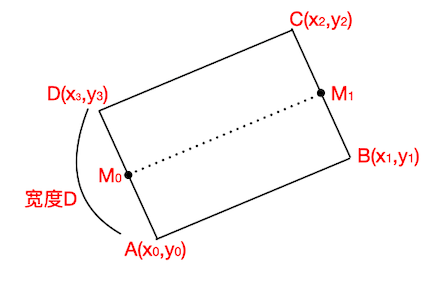
\includegraphics[width=12cm]{figures/obstacle_bottom.png}
    \caption{障碍物底面}
    \label{fig:obstacle_bottom}
\end{figure}
\par 特别注意特殊判断长宽平行与轴的情况,此时可以直接通过$M_0,M_1$的坐标计算四个顶点的坐标,即四个顶点的坐标分别为$(x_0,y_0-\dfrac{D}{2}),(x_0,y_0+\dfrac{D}{2}),(x_1,y_1-\dfrac{D}{2}),(x_1,y_1+\dfrac{D}{2})$。
具体的代码如图\ref{code:obstacle_vertice_process},通过if-else判断情况来具体计算,最后通过重载结构体的读入来实现使用c++的cin就可以读入障碍物数据时计算顶点并存储在结构体当中,方便后续使用。
其中结构体当中的conveyByPrec函数是将原始数据下的障碍物离散到指定precision精度下的处理后的障碍物。
\lstinputlisting[style=C++,caption={顶点处理},label=code:obstacle_vertice_process]{code/obstacle_vertice_process}
\par 通过处理数据,使得可以将最短路径算法应用在三维空间当中,通过控制离散化的精度来实现控制最短路径的精度,离散后格点的标记来实现不可访问情况的判断,达到将实际空间离散化到指定精度的理想空间,从而计算出格点组成的最短路径。

\subsection{相交判断}
\par 通过计算出格点组成的最短路径后,由于存在三角形定则,即三角形两边之和大于第三边,所以在计算的格点路径后,是可以通过运用三角形定则拟合计算出更短的路径,此时就需要判断所拟合的新路径是否经过了障碍物。此时问题可以抽象为线段与长方体是否相交的判定问题,根据线段的向量表示法,有线段$\vec{PQ}$:$P+k(Q-P),k\in [0,1]$,若存在与某个障碍物相交的情况,即存在k属于0~1之间,使得该点在障碍物之内。
考虑障碍物:底面$A(x_0,y_0),B(x_1,y_1),C(x_2,y_2),D(x_3,y_3)$,高的范围$[z_0,z_1]$。由于障碍物的高与z轴平行,故只需要考虑该障碍物由无数个矩形在z轴上堆叠而成。首先,我们讨论如何判断一个二维点坐标是否位于底面矩形当中,设该点坐标为$E(x,y)$,若该点在矩形内,则满足$\vec{AB}\times\vec{AE}*\vec{CD}\times\vec{CE}\ge 0$,若该式子成立则说明该点在边AB和边CD之间;同理,还需要成立$\vec{DA}\times\vec{DE}*\vec{BC}\times\vec{BE}\ge 0$,即该点在边DA和BC之间。两个条件需要同时满足,则说明该点在四条边之内,即在该矩形范围内。
\par 将问题放大到三维空间当中,该线段若与该障碍物有交点,则至少存在一个可行的k解满足E的坐标在障碍物内,则我们求出要与该障碍物相交时k值所取的范围,若存在有效范围,则表明该线段与该障碍物相交。
首先,对于z轴相交,设$\vec{R}=PQ=Q-P$为向量$PQ$的方向向量,则k的范围应在$k\in [0,1]$,对于障碍物的z轴所计算的k的取值为:$k_0=\dfrac{z_0-P.z}{R.z},k_1=\dfrac{z_1-P.z}{R.z}$,若$R.z<0$小于0时交换$k_0,k_1$的值。则$k_0\leq k_1$存在z轴可行解,否则无解。代码如下\ref{code:check_insect_zaxis},首先初始化k取值范围为[0,1],通过分别计算$z_0,z_1$对应的k取值来更新。
\lstinputlisting[style=C++,caption={计算z轴k取值},label=code:check_insect_zaxis]{code/check_insect_zaxis}
对于x、y所决定的k值的范围,需要计算的是该点在矩形内部的情况,则可以用到之前我们所讨论到的公式
\begin{equation}
    \vec{AB}\times\vec{AE}*\vec{CD}\times\vec{CE}\ge 0
\label{con:innerABandCD}
\end{equation}
和
\begin{equation}
    \vec{DA}\times\vec{DE}*\vec{BC}\times\vec{BE}\ge 0
\label{con:innerDAandBC}
\end{equation}
公式\ref{con:innerABandCD}和\ref{con:innerDAandBC}两者需要同时成立。针对可能出现该点在xy平面内是一个点的情况,即一条平行与z轴的线段,此时利用公式\ref{con:innerABandCD}和\ref{con:innerDAandBC}对该点做一个计算,若两公式都满足则说明该线段在xy平面的点在障碍物底面中之中,该部分代码如下\ref{code:check_insect_onepoint}。
\lstinputlisting[style=C++,caption={相交时单点的情况},label=code:check_insect_onepoint]{code/check_insect_onepoint}
对于线段$\vec{PQ}$能到达的点坐标E,有$E(P.x+k(Q.x-P.x),P.y+k(Q.y-P.y))$。将该点E坐标代入公式\ref{con:innerABandCD}中有
\begin{align*} 
    \vec{AB}\times\vec{AE} = {}& (x_1-x_0,y_1-y_0)\times(P.x+k(Q.x-P.x)-x_0,P.y+k(Q.y-P.y)-y_0) \\ 
    = {}& [(x_1-x_0)(Q.y-P.y)-(Q.x-P.x)(y_1-y_0)]k  \\ 
    &{} +(x_1-x_0)(P.y-y_0)-(P.x-x_0)(y_1-y_0) 
\end{align*}
我们设k的系数$a_1=(x_1-x_0)(Q.y-P.y)-(Q.x-P.x)(y_1-y_0)$,后的常数为$b_1=(x_1-x_0)(P.y-y_0)-(P.x-x_0)(y_1-y_0)$,则公式可化简为$\vec{AB}\times\vec{AE} = a_1k+b_1$。
\begin{align*} 
    \vec{CD}\times\vec{CE} = {}& (x_3-x_2,y_3-y_2)\times(P.x+k(Q.x-P.x)-x_2,P.y+k(Q.y-P.y)-y_2) \\ 
    = {}& [(x_3-x_2)(Q.y-P.y)-(Q.x-P.x)(y_3-y_2)]k  \\ 
    &{} +(x_3-x_2)(P.y-y_2)-(P.x-x_2)(y_3-y_2) 
\end{align*}
设k的系数为$a_2=(x_3-x_2)(Q.y-P.y)-(Q.x-P.x)(y_3-y_2)$,后的常数为$b_2=(x_3-x_2)(P.y-y_2)-(P.x-x_2)(y_3-y_2)$,则公式可化简为$\vec{CD}\times\vec{CE} = a_2k+b_2$。
则$\vec{AB}\times\vec{AE}*\vec{CD}\times\vec{CE}\ge 0$等价于方程$(a_1k+b_1)*(a_2k+b_2) \ge 0 = a_1a_2x^2+(a_1b_2+a_2b_1)x+b_1b_2 \ge 0$,即是二次函数求解的问题。
关于二次函数根求解的问题,我们需要讨论系数是否为0,以及特判二次函数出现非实数解的情况。若不存在这些情况,则对于二次函数$y=ax^2+bx+c$,二次函数根的计算公式:
\begin{equation}
    x=\dfrac{-b\pm\sqrt{b^2-4ac}}{2a}
\label{con:Quadratic_functions}
\end{equation}
故我们将公式\ref{con:Quadratic_functions}应用在方程$a_1a_2x^2+(a_1b_2+a_2b_1)x+b_1b_2 \ge 0$上,可以得到该方程的解为
\begin{equation}
    k=\dfrac{-(a_1b_2+a_2b_1)\pm\sqrt{(a_1b_2+a_2b_1)^2-4a_1a_2b_1b_2}}{2a_1a_2}
\label{con:kBaseOnQuadFun}
\end{equation}
我们将之前假设的$a_1,a_2,b_1,b_2$代入该公式既可以求出对于公式\ref{con:innerABandCD}限制下k的取值范围。使用该求解值更新基于z范围求出的k范围,若新的$k_0\leq k_1$则存在可行解,否则无解。代码如下\ref{code:check_insect_firstcross},代码首先判断了出现系数为0时二次函数退化为一次函数的情况,下文将进行分析,否则计算二次函数对应的k值用来更新并判断。
\lstinputlisting[style=C++,caption={公式\ref{con:innerABandCD}求解k值},label=code:check_insect_firstcross]{code/check_insect_firstcross}
\par 对于公式\ref{con:innerDAandBC},相似的有,我们将点E坐标代入有
\begin{align*} 
    \vec{DA}\times\vec{DE} = {}& (x_0-x_3,y_0-y_3)\times(P.x+k(Q.x-P.x)-x_3,P.y+k(Q.y-P.y)-y_3) \\ 
    = {}& [(x_0-x_3)(Q.y-P.y)-(Q.x-P.x)(y_0-y_3)]k  \\ 
    &{} +(x_0-x_3)(P.y-y_3)-(P.x-x_3)(y_0-y_3) 
\end{align*}
同样的,设k的系数$a_1=(x_0-x_3)(Q.y-P.y)-(Q.x-P.x)(y_0-y_3)$,后的常数为$b_1=(x_0-x_3)(P.y-y_3)-(P.x-x_3)(y_0-y_3)$,则公式可化简为$\vec{DA}\times\vec{DE} = a_1k+b_1$。
\begin{align*} 
    \vec{BC}\times\vec{BE} = {}& (x_2-x_1,y_2-y_1)\times(P.x+k(Q.x-P.x)-x_1,P.y+k(Q.y-P.y)-y_1) \\ 
    = {}& [(x_2-x_1)(Q.y-P.y)-(Q.x-P.x)(y_2-y_1)]k  \\ 
    &{} +(x_2-x_1)(P.y-y_1)-(P.x-x_1)(y_2-y_1) 
\end{align*}
设k的系数为$a_2=(x_2-x_1)(Q.y-P.y)-(Q.x-P.x)(y_2-y_1)$,后的常数为$b_2=(x_2-x_1)(P.y-y_1)-(P.x-x_1)(y_2-y_1)$,则公式可化简为$\vec{CD}\times\vec{CE} = a_2k+b_2$。
故我们将新的$a_1,a_2,b_1,b_2$的值代入公式\ref{con:kBaseOnQuadFun}中计算出对于公式\ref{con:innerDAandBC}限制下的k的取值范围。使用新求解的k值更新由公式\ref{con:innerABandCD}更新的k值,若最后求解的k值仍满足$k_0\leq k_1$,则说明线段$PQ$存在与该障碍物相交的情况。
具体代码如下\ref{code:check_insect_secondcross},代码同样先判断了退化的情况,再计算的二次函数对应k取值来更新并判断。若最后更新后的k取值仍满足$k_0\leq k_1$,则说明存在可行k解使得存在该线段$PQ$与障碍物相交,此时代码true表示产生碰撞。
\lstinputlisting[style=C++,caption={公式\ref{con:innerDAandBC}求解k值},label=code:check_insect_secondcross]{code/check_insect_secondcross}
\par 针对可能出现的二次函数系数为0的情况,即公式退化为一次函数的正负问题,如$b_1(a_2k+b_2)\ge 0$,此时特判系数为0的各种情况,计算一次函数下k的取值即可,代码如图\ref{code:check_insect_firstcross}的8行至20行。对于出现非实数解的情况,即$\Delta=b^2-4ac<0$时,此时表明不存在有效k的取值的点使之在障碍物内,故该线段与障碍物不相交。
\par 至此,已经完成了三维空间内线段与障碍物相交的讨论,利用通过离散化格点求解的格子点路径,不断检查格子点之间是否存在不与障碍物相交也能相连且距离更短的情况,来进一步优化路径。

\subsection{最短路径算法}
\par 三维空间最短路径算法的实现,在指定精度后,将实际空间离散到指定精度的空间,因此算法需要求解出离散空间中从起点到终点的格点最短路径,再利用上述讨论的相交算法来拟合路径,最后给出该精度下近似的最短路径和所通过的格点线段。

\subsubsection{基于BFS的三维最短路径算法}
\par 广度优先搜索(BFS)算法,又叫做宽度优先搜索,是一种在图上的搜索算法。算法将从根节点开始,沿着树的宽度遍历树的节点。在图上时,可以视为根节点为起点的一棵树。BFS是一种暴力算法,目的是系统的展开并检查图中的所有节点,以找寻结果。算法的实现一般采用open-closed表,所有因为展开节点而得到都会被加进一个先进先出的队列中,其邻居节点尚未检验的节点会被存放在一个称为open的容器,而被检验过的节点则被存放在被称为closed的容器中。其实现方法为:
\begin{enumerate}
    \item 首先将根节点放在队列中。
    \item 从队列中取出现在的第一个节点,并检查。
    \begin{itemize}
        \item 如果找到目标,则结束搜索并返回结果。
        \item 否则将它所有还没有检查过的相邻子节点加入队列中。
    \end{itemize}
    \item 若队列为空,表示检查了所有点都没有找到目标。结束搜索并返回未找到目标。
    \item 重复步骤2.
\end{enumerate}
\par 在离散后的三维空间中,将把每一个整数格点视为顶点,即$V=\{v_i(x,y,z)|x\in N,y\in N,z\in N\}$,则对于顶点$v_1=(x,y,z)$相邻的顶点有分别在x轴、y轴、z轴相邻的6个顶点:$(x-1,y,z),(x+1,y,z),(x,y-1,z),(x,y+1,z),(x,y,z-1),(x,y,z+1)$。
则基于BFS的三维空间最短路径算法实现,是基于从起点格点逐渐向外发散并记录所经过的路径,直到找到终点。算法需要遍历大量的点,若起点$st(x_0,y_0,z_0)$与终点$ed(x_1,y_1,z_1)$之间三维坐标差的最大值为$n=max\{x_1-x_0,y_1-y_0,z_1-z_0\}$,则算法至少需要遍历$n^3$个点,则算法的时间复杂度为$O(n^3)$,空间复杂度为$O(n^3)$。
搜索算法初始化部分如代码\ref{code:bfs_init}所示,首先定义了距离向量dist,用来存储起点距离该格点的最短路径的长度;方向向量dir,用来找到现在顶点相邻的顶点;以及使用数组q和指针front和rear实现队列的功能,并能将顶点保存起来用来回溯路径;pre数组存储该顶点nowNode的前驱顶点preNode,即是BFS时nowNode是通过preNode搜索到的且经过格子点数量最少的情况时的前驱顶点。
\lstinputlisting[style=C++,caption={BFS搜索算法初始化代码},label=code:bfs_init]{code/bfs_alorithm_init}
\par 初始化完成后,算法使用数组实现的队列q,front指针表示当前节点在队列中的位置,rear指针表示队列的最后一个节点的位置,当$front\leq rear$时表示队列不为空。则算法通过不断取出队列的当前节点,并检查是否为终点,或者跳过路径长度以及大于了已经找到的最短路径长度的节点,对搜索做剪枝。随后遍历该节点的相邻节点,若相邻节点没有超出边界且可以访问,则更新其距离向量,并将其加入到队列中。
\lstinputlisting[style=C++,caption={BFS搜索算法主要函数},label=code:bfs_main]{code/bfs_alorithm}
\par 若算法返回true则代表至少存在一条从起点格点到终点格点的格点最短路径,此时需要我们对路径做一个拟合,进一步优化路径长度。根据上述障碍物相交判断中所实现的函数check\_insect做该条路径上顶点到顶点的拟合操作,即若直接在这两个顶点之间连成线段不经过障碍物且距离更短则直接连接这两个顶点为一条线段而不经过中途格点。此时拟合算法所需要的时间与所找到的最短路径长度有关,对于BFS搜索算法,平均最短路径上的格子节点数量在kn个,即n的常数级别的个数。
由于路径上的每个顶点都至多与路径上的所有顶点做一次障碍物相交判断算法,且使用一个长度为路径上的顶点个数的数组作为距离向量,则算法的时间复杂度在$O(n^2)$,空间复杂度为$O(n^2)$。
具体的代码如代码\ref{code:bfs_checkinsect},check\_segement\_cross\_all\_obstacles(P,Q)是对所有的障碍物做相交判断,若出现与一个障碍物与该线段$\vec{PQ}$相交则返回非-1,算法通过使用定义的pre数组逐渐找到整条路径并记录到tmp链表中,对每找出的一条路径做一次拟合,dp\_dist记录该条路径上顶点的距离向量,若此条路径长度更短,则记录在path链表中。
\lstinputlisting[style=C++,caption={BFS搜索算法拟合路径},label=code:bfs_checkinsect]{code/bfs_checkinsect}
\par 至此已经完成了使用BFS算法对三维空间带有障碍物寻找最短路径的设计和实现,如分析中拟合算法的时间复杂度平均为$O(n^2)$会小于寻路算法的时间复杂度$O(n^3)$,拟合算法的空间复杂度$O(n^2)$会小于寻路算法的空间复杂度$O(n^3)$,因此整个算法的时间复杂度和空间复杂度都为$O(n^3)$。当时间空间较大或离散精度较大时,整个算法运行时间和占用空间不太理想。

\subsubsection{基于A*的三维最短路径算法}
\par 正如章节\ref{section:A*algorithm_exp}中对A*算法的分析,由于A*算法采用了估价函数h(n)进行启发式搜索,提高了找到路径的时间和空间的效率,并且可以保证找到基于估价函数的最优路径。对于估价函数h(n),我们采用欧几里得距离,即$nowNode(x_0,y_0,z_0),\\endNode(x_1,y_1,z_1)$之间的欧几里得距离为$d(nowNode,endNode)=\\\sqrt{(x_0-x_1)^2+(y_0-y_1)^2+(z_0-z_1)^2}$。则g(n)表示的是起点到任意顶点n的最短路径长度,估算函数即为f(n)=g(n)+h(n)。
代码如代码\ref{code:astar_init}所示,结构体heap\_node用来存储函数$f(n)$和当前节点在队列中的索引,并重载了小于和大于运算符配合优先队列priority\_queue以实现大顶堆;链表arr记录的是队列遍历的点,dist向量存储的是该点的最短路径长度,pre向量存储的是该点在最短路径中前驱节点的编号,paths链表存储的是最后计算出的最短路径所经过的格子节点,record哈希表存储的是三维空间内的格子点对应在队列元素arr中的索引,\_\_init\_\_函数实现算法的初始化操作。
\lstinputlisting[style=C++,caption={A*算法初始化},label=code:astar_init]{code/astar_init}
A*算法每次从队列中找出f(n)值最小的顶点,将其作为当前顶点,去遍历其周围的顶点,由于顶点到顶点之间的边权是欧几里得距离,故可以应用Dijkstra算法的松弛操作,遍历顶点时计算出该点到已经计算过的点(即arr链表存储的点)之间不经过障碍物的距离,即将原来的拟合算法与寻路算法合并在了一起,代码如代码\ref{code:astar_main}所示,\_\_build\_\_是寻路并拟合的函数,\_\_process\_\_是处理最短路径并输出的函数,\_\_main\_\_是算法入口。
\lstinputlisting[style=C++,caption={A*算法主要函数},label=code:astar_main]{code/astar_main}
\par 由于A*算法属于启发式算法,对于其复杂度的分析不太准确,但已知的是由于估价函数的存在,可以使路径朝终点方向搜索,有效地减少遍历点的数量,从而在时间和空间复杂度上都有不小的优化。

\section{本章总结}
\par{\kaishu 本章主要讨论了算法实现当中的重要部分的实现原理,首先分析了常用的最短路径Dijkstra和A*算法,对其原理和实现方法进行了分析,以及介绍了对障碍物数据进行处理的算法和线段与障碍物相交算法,最后就是讨论关于基于BFS和A*最短路径算法的实现。
在常见的正权图结构中,Dijkstra算法拥有非常好的时间和空间复杂度,而引入了估价函数的A*算法,在进行启发式搜索提高搜索算法效率的同时,可以保证找到一条基于评估函数的最优路径。
对于输入的数据,我们需要先对输入的障碍物底面的两中点和z轴范围做一个处理,计算出其的底面四个顶点。在起点、终点和障碍物离散到指定精度的空间后,提出了利用了向量叉积来检查线段是否与障碍物相交的算法。
最后设计和实现了基于BFS和A*的三维空间最短路径算法,并分析了两者的特点,BFS算法原理较为简单,是基于暴力的系统展开并检查图中的所有顶点;A*算法采用了估价函数,可以大大提高算法使用的运行时间和减小空间占用,并且能找到一条基于估价函数的最优路径。}

\chapter{算法测试}
\par 为了测试算法的正确性,需要用尽可能全面的数据样例来测试。根据算法构成,设计了数据对数据处理算法模块、路径求解算法模块以及整体算法进行测试。障碍物数据分为输入的原始数据,以底面平行边的两中点$M_0,M_1$、底面边长D和z轴范围$z_0,z_1$给出,格式为[$M_0$, $M_1$], D, [$z_0$, $z_1$];处理后的障碍物数据为离散到指定精度后的底面四顶点A、B、C、D的坐标以及z轴范围,格式为[A, B, C, D], [$Z_0$, $Z_1$]。效果显示使用Matlab绘制出障碍物与起点到终点所经过的路径,可以直观的看出算法寻路效果 \cite{r7}。

\section{数据处理算法测试}
\par 对数据处理模块而言,算法代码主要是代码\ref{code:obstacle_vertice_process},即将输出的数据信息格式化到可以供后续算法使用的格式,主要是关于计算障碍物底部四个顶点和将顶点离散到指定精度下。测试数据如表\ref{tab:process_input_test_data1}。
\begin{table}[htb]
    \centering
    \caption{输入测试数据1}
    \label{tab:process_input_test_data1}
    \begin{tabular}{cccc}
        \toprule
        起点&终点&障碍物&精度\\
        \midrule
        (0, 0, 0)&(5, 5, 5)&(0.5, 0.5), (3.7, 3.7), 1, [0.2, 4]&0.1\\
        \bottomrule
    \end{tabular}
\end{table}
测试数据为起点终点经过了单个障碍物的情况,此时障碍物信息如表\ref{tab:process_input_test_data1_obstacle1}。障碍物底面是由中点为(0.5, 0.3),(3.7, 3.7),边长为1的矩形组成,高度z轴范围为[0.2, 4]。
\begin{table}[htb]
    \centering
    \caption{障碍物1信息}
    \label{tab:process_input_test_data1_obstacle1}
    \begin{tabular}{ccc}
        \toprule
        底面平行边的两中点&底面边长&z轴范围\\
        \midrule
        (0.5, 0.5) (3.7, 3.7)&1&[0.2, 4]\\
        \bottomrule
    \end{tabular}
\end{table}
根据算法\ref{code:obstacle_vertice_process},计算出障碍物的数据为四顶点的坐标分别为(0.146447, 0.853553), (3.34645, 4.05355), (4.05355, 3.34645), (0.853553, 0.146447),此时,使用Matlab绘制出关于此障碍物的图像,图像如图\ref{fig:obstacle_ex_bottom}。
\begin{figure}[htb]
    \centering
    \caption{数据处理测试障碍物底面}
    \label{fig:obstacle_ex_bottom}
    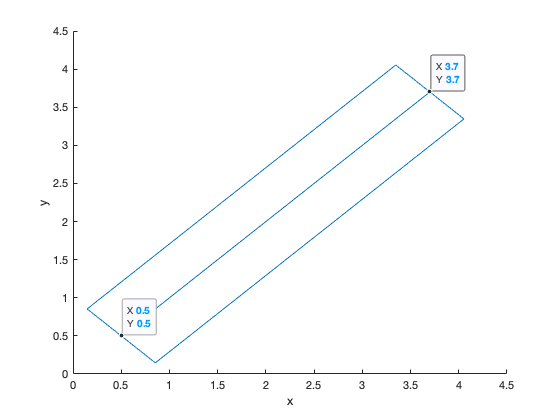
\includegraphics[width=10cm]{figures/obstacle_ex_bottom.png}
\end{figure}
\par 验证图示底面是否满足障碍物底面,底面边长为$d=\\\sqrt{(0.146447-0.853553)^2+(0.853553-0.146447)^2}=\sqrt{0.999997790436}\approx 1$,在误差范围内满足相等;
若两边垂直,满足$L_1\cdot L_2=0$,$\vec{AB}=(0.853553, 0.146447)-(0.146447, 0.853553)=(0.707106,-0.707106)$,$\vec{M_0M_1}=(3.7,3.7)-(0.5,0.5)=(3.2,3.2)$,则$\vec{AB}\cdot\vec{M_0M_1}=0.707106\times3.2-0.707106\times3.2=0$,说明边$AB$与中点连线$M_0M_1$相垂直;
再验证相邻边是否垂直,$\vec{BC}=(4.05355, 3.34645)-(0.853553, 0.146447)=(3.199997,3.200003)$,则此时$\vec{AB}\cdot\vec{BC}=0.707106\times3.199997-0.707106\times3.200003\approx0$,说明相邻边垂直。
将计算顶点后的该障碍物在Matlab中绘制出来如图\ref{fig:obstacle_ex}。完成对障碍物顶点的计算之后,算法还将会对数据进行离散到指定精度下的操作,即$(\lfloor\dfrac{x}{precision}\rfloor,\lfloor\dfrac{y}{precision}\rfloor,\lfloor\dfrac{z}{precision}\rfloor)$。此时精度指定为0.1,故离散后的障碍物数据为底面矩形顶点为[(1, 8), (33, 40), (40, 33), (8, 1)],z轴范围为[2, 40]。出发点(0,0,0)离散后仍为(0,0,0),终点(5,5,5)离散后为(50,50,50)。
\begin{figure}[htb]
    \centering
    \caption{测试障碍物}
    \label{fig:obstacle_ex}
    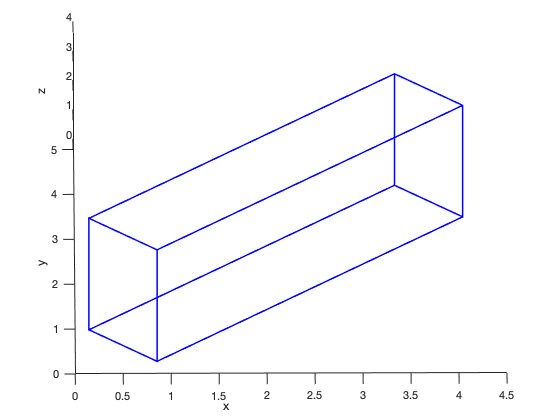
\includegraphics[width=12cm]{figures/obstacle_ex.png}
\end{figure}

\section{路径求解算法测试}
\par 关于路径求解算法的正确性测试,主要是障碍物碰撞检查算法和路径寻找算法正确性的测试,且数据为完成障碍物计算并离散到指定精度下的数据,障碍物碰撞检查算法主要是公式\ref{con:innerABandCD}和\ref{con:innerDAandBC}的应用,路径寻找算法是应用BFS或A*算法在指定精度下寻找格点路径,路径拟合算法是通过结合路径寻找算法和障碍物碰撞检测算法从而找到一条最短的路径。
数据采用上述表\ref{tab:process_input_test_data1}中关于障碍物计算算法测试的数据,首先起点P(0,0,0)到终点Q(50,50,50)的线段与障碍物的关系如图\ref{fig:insect_ex_insected},此时线段是与障碍物相交的,即不可以直接到达的情况。
\begin{figure}[htb]
    \centering
    \caption{障碍物与起点到终点线段的关系}
    \label{fig:insect_ex_insected}
    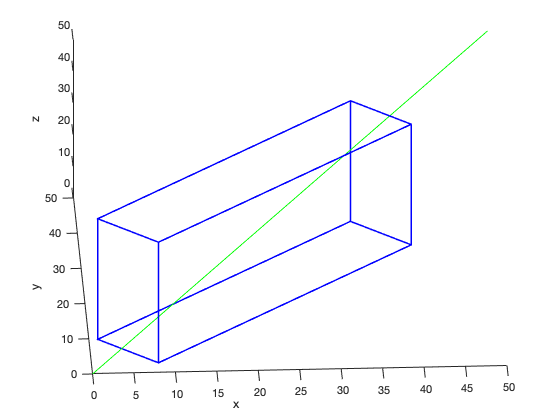
\includegraphics[width=12cm]{figures/insect_ex_insected.png}
\end{figure}
将线段$\vec{PQ}=P+k\cdot PQ=(0,0,0)+k(50-0,50-0,50-0)=(50k,50k,50k)$和障碍物代入障碍物碰撞检查算法进行测试,步骤如下:
\begin{enumerate}
    \item 初始化可行解k范围为[0,1];
    \item 对障碍物的z取值进行计算,由$k_i=\dfrac{z_i}{50k}$解得新的可行解范围[0.04,0.8];
    \item 对障碍物进行公式\ref{con:innerABandCD}检查,计算得到系数、常数分别为$a_1=0,b_1=-224,a_2=0,b_2=-224$,此时退化为一次函数,由于$b_1b_2>0$可知满足公式,此时不对k范围做更新;
    \item 对障碍物进行公式\ref{con:innerDAandBC}检查,计算得到系数、常数分别为$a_1=-700,b_1=63,a_2=700,b_2=-511$,此时$\Delta=98344960000>0$,解的新k的取值为[0.09,0.73];
    \item 综上,存在k的有效范围为[0.09,0.73],故线段PQ与障碍物相交;
\end{enumerate}
\par 对寻路算法进行测试,使用算法对该起点、终点和障碍物进行寻路操作,此时找到的拟合格点路径所经过点如图\ref{fig:find_path_ex_out}。
\begin{figure}[htb]
    \centering
    \caption{寻路算法测试输出}
    \label{fig:find_path_ex_out}
    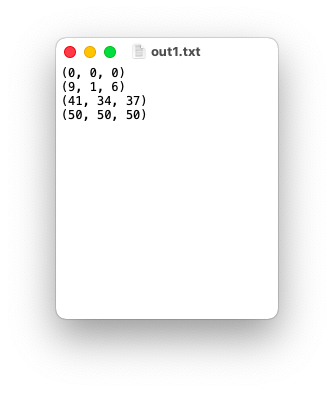
\includegraphics[width=8cm]{figures/find_path_ex_out.png}
\end{figure}
此时,根据算法输出结果,将经过格点数据和障碍物在Matlab中绘制出来,如图\ref{fig:find_path_ex_paint}。此时可知该拟合路径满足不与障碍物相交的情况下,路径长度最短的条件。
\begin{figure}[htb]
    \centering
    \caption{寻路算法测试路径与障碍物关系}
    \label{fig:find_path_ex_paint}
    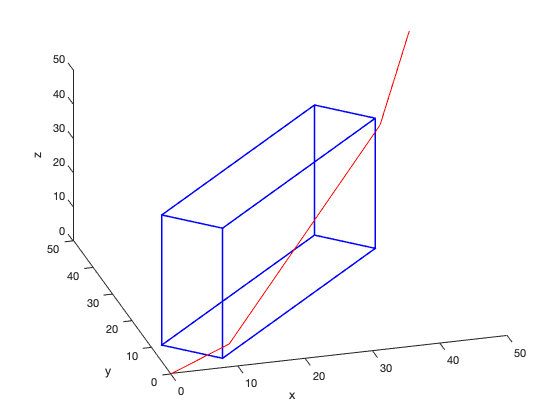
\includegraphics[width=10cm]{figures/find_path_ex_paint.png}
\end{figure}

\section{综合测试}
\par 完成对算法包含的主要模块:数据处理算法、路径求解算法的测试之后,还需要对整个算法进行全面的样例测试,需要包含多个场景,常见或稀有场景,以测试算法的稳定性。

\subsection{常见室内场景}
\par 常见室内场景,其中包含沙发、板凳、电视和冰箱等物体,根据图\ref{fig:test_common_situation_reality}中所示实际空间,建模数据为表\ref{tab:test_common_situation_data},其中包含5个障碍物。
\begin{figure}[htb]
    \centering
    \caption{常见室内空间图}
    \label{fig:test_common_situation_reality}
    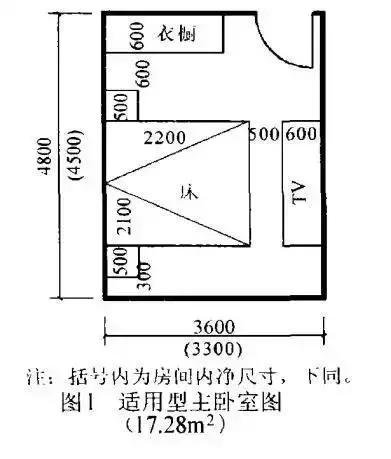
\includegraphics[width=10cm]{figures/test_common_situation_reality.JPG}
\end{figure}
\begin{table}[htb]
    \centering
    \caption{常见室内空间测试数据}
    \label{tab:test_common_situation_data}
    \begin{tabular}{cccc}
        \toprule
        起点&终点&障碍物&精度\\
        \midrule
        \multirow{5}*{(2, 0, 0)}&\multirow{5}*{(0.1, 5, 0.1)}&(0.25, 0.3), (0.25, 0.8), 0.5, [0, 0.5]&\multirow{5}*{0.1}\\
        ~&~&(1.1, 0.8), (1.1, 2.9), 2.2, [0, 0.5]&~\\
        ~&~&(0.25, 2.9), (0.25, 3.4), 0.5, [0, 0.5]&~\\
        ~&~&(0.9, 4), (0.9, 4.5), 1.8, [0, 2]&~\\
        ~&~&(3, 0.8), (3, 2.9), 0.6, [0, 1]&~\\
        \bottomrule
    \end{tabular}
\end{table}
对数据完成预处理并离散到指定精度0.1后,得到离散后数据为表\ref{tab:test_common_situation_processed_data},此时将建模后的数据在Matlab中绘制的模型俯视图和侧视图如图\ref{fig:test_common_situation_pic_top}和图\ref{fig:test_common_situation_pic_lean}。
\begin{table}[htb]
    \centering
    \caption{常见室内空间处理后数据}
    \label{tab:test_common_situation_processed_data}
    \begin{tabular}{ccc}
        \toprule
        起点&终点&障碍物\\
        \midrule
        \multirow{5}*{(20, 0, 0)}&\multirow{5}*{(1, 50, 1)}&[(0, 2), (5, 2), (5, 8), (0, 8)], [0, 5]\\
        ~&~&[(0, 8), (22, 8), (22, 28), (0, 28)], [0, 5]\\
        ~&~&[(0, 28), (5, 28), (5, 34), (0, 34)], [0, 5]\\
        ~&~&[(0, 40), (18, 40), (18, 45), (0, 45)], [0, 20]\\
        ~&~&[(27, 8), (32, 8), (32, 28), (27, 28)], [0, 10]\\
        \bottomrule
    \end{tabular}
\end{table}
\begin{figure}[htb]
    \centering
    \caption{常见室内空间处理后建模-俯视图}
    \label{fig:test_common_situation_pic_top}
    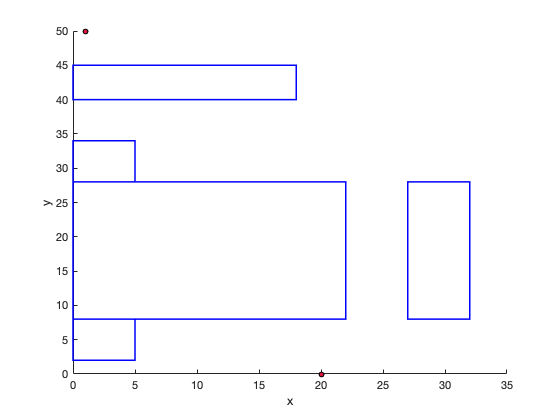
\includegraphics[width=10cm]{figures/test_common_situation_pic_top.png}
\end{figure}
\begin{figure}[htb]
    \centering
    \caption{常见室内空间处理后建模-侧视图}
    \label{fig:test_common_situation_pic_lean}
    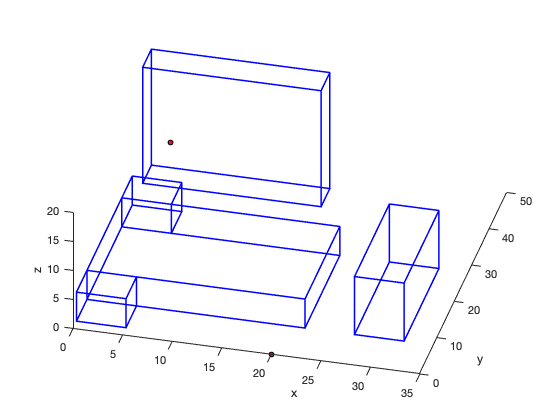
\includegraphics[width=10cm]{figures/test_common_situation_pic_lean.png}
\end{figure}
对数据进行寻路操作,设定起点为(2, 0, 0),终点为(0.1, 5, 0.1),离散在指定精度后起点为(20, 0, 0),终点为(1, 50, 1),算法得到的输出如图\ref{fig:test_common_situation_out},包含了起点、终点信息,障碍物信息以及最短路径通过的格点信息。将障碍物信息和路径信息使用Matlab绘制出来的模型的俯视图和侧视图分别如图\ref{fig:test_common_situation_out_top}和图\ref{fig:test_common_situation_out_lean},此时路径合法不经过障碍物并且满足路径长度最短。
\begin{figure}[htb]
    \centering
    \caption{常见室内空间最短路径经过顶点}
    \label{fig:test_common_situation_out}
    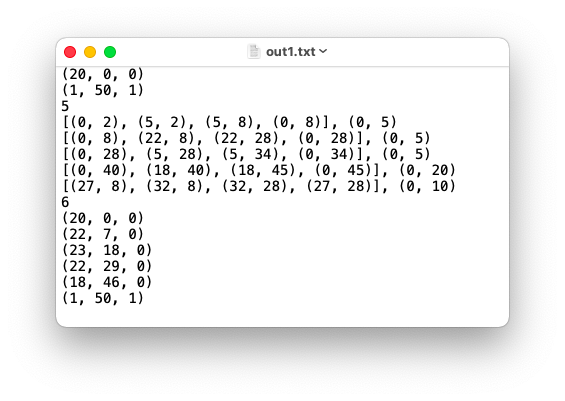
\includegraphics[width=10cm]{figures/test_common_situation_out.png}
\end{figure}
\begin{figure}[htb]
    \centering
    \caption{常见室内空间最短路径结果-俯视图}
    \label{fig:test_common_situation_out_top}
    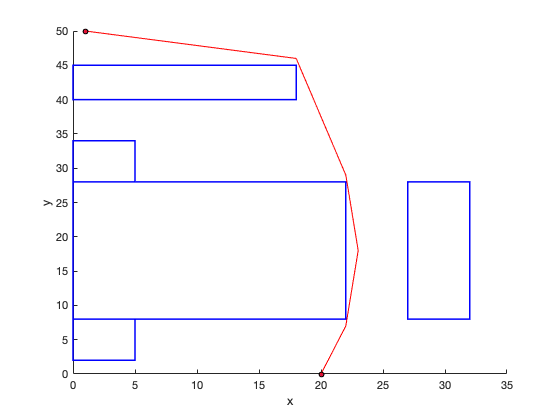
\includegraphics[width=10cm]{figures/test_common_situation_out_top.png}
\end{figure}
\begin{figure}[htb]
    \centering
    \caption{常见室内空间最短路径结果-侧视图}
    \label{fig:test_common_situation_out_lean}
    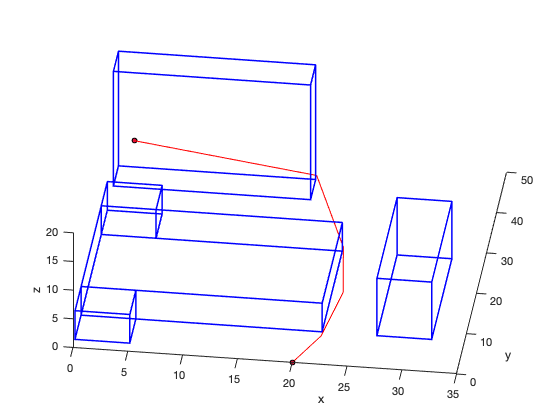
\includegraphics[width=10cm]{figures/test_common_situation_out_lean.png}
\end{figure}

\subsection{复杂室内场景}
\par 考虑在简单室内场景的基础上,增加障碍物数量和路线的复杂度,因此建模为两个房屋相邻的情况,从一个房屋到另一个房屋内的最短路径求解情况。
此时重复简单室内场景建模,原始数据为表\ref{tab:test_complex_situation_data},对其完成离散到指定精度0.1后,得到离散后的数据如表\ref{tab:test_complex_situation_processed_data},此时将处理后数据使用Matlab绘制出来可得图像的俯视图和侧视图分别为图\ref{fig:test_common_situation_processed_pic_top}和图\ref{fig:test_common_situation_processed_pic_lean}。
由建模图像可知,封闭的房屋有门和窗两处开口,此时设计出发点在左侧房间内,为(3, 0, 0),离散后为(30, 0, 0);终点在右侧房间内,为(7, 0, 0),离散后为(70, 0, 0)。所以若存在路线,应该是从左侧门进入左侧房间,通过左侧窗口离开左侧房间,再通过右侧窗口进入右侧房间,最后达到右侧门口的终点位置。使用算法在处理后的空间求出起点到终点的最短路径,此时算法输出的结果如图\ref{fig:test_complex_situation_out},其中同样包括起点、终点、障碍物信息和路径经过的顶点信息。
将输出信息使用Matlab绘制成图像,此时最短路径经过的路线图像的俯视图和侧视图分别为图\ref{fig:test_complex_situation_out_top}和图\ref{fig:test_complex_situation_out_lean},可以看出此路径满足没有经过障碍物且路径最短的条件。
\begin{table}[htb]
    \centering
    \caption{复杂室内空间测试数据}
    \label{tab:test_complex_situation_data}
    \begin{tabular}{cccc}
        \toprule
        起点&终点&障碍物&精度\\
        \midrule
        \multirow{20}*{(3, 0, 0)}&\multirow{20}*{(7, 0, 0)}&(1.35, 0), (1.35, 0.1), 2.7, [0, 2]&\multirow{20}*{0.1}\\
        ~&~&(1.65, 0), (1.65, 0.1), 3.3, [2, 2.5]&~\\
        ~&~&(0.25, 0.3), (0.25, 0.8), 0.5, [0, 0.5]&~\\
        ~&~&(3.3, 0), (3.3, 4.8), 0.1, [0, 2.5]&~\\
        ~&~&(0.05, 0), (0.05, 4.8), 0.1, [0, 2.5]&~\\
        ~&~&(1.7, 0), (1.7, 4.9), 3.3, [2.5, 2.6]&~\\
        ~&~&(1.7, 4.8), (1.7, 4.9), 3.3, [0, 2]&~\\
        ~&~&(1.9, 4.8), (1.9, 4.9), 2.8, [2, 2.5]&~\\
        ~&~&(1.1, 0.8), (1.1, 2.9), 2.2, [0, 0.5]&~\\
        ~&~&(0.25, 2.9), (0.25, 3.4), 0.5, [0, 0.5]&~\\
        ~&~&(0.9, 4), (0.9, 4.5), 1.8, [0, 2]&~\\
        ~&~&(3, 0.8), (3, 2.9), 0.6, [0, 1]&~\\
        ~&~&(5.35, 0), (5.35, 0.1), 2.7, [0, 2]&~\\
        ~&~&(5.65, 0), (5.65, 0.1), 3.3, [2, 2.5]&~\\
        ~&~&(4.25, 0.3), (4.25, 0.8), 0.5, [0, 0.5]&~\\
        ~&~&(7.3, 0), (7.3, 4.8), 0.1, [0, 2.5]&~\\
        ~&~&(4, 0), (4, 4.8), 0.1, [0, 2.5]&~\\
        ~&~&(5.7, 0), (5.7, 4.9), 3.3, [2.5, 2.6]&~\\
        ~&~&(5.7, 4.8), (5.7, 4.9), 3.3, [0, 2]&~\\
        ~&~&$\vdots$&~\\
        \bottomrule
    \end{tabular}
\end{table}
\begin{table}[htb]
    \centering
    \caption{复杂室内空间处理后测试数据}
    \label{tab:test_complex_situation_processed_data}
    \begin{tabular}{ccc}
        \toprule
        起点&终点&障碍物\\
        \midrule
        \multirow{20}*{(2, 0, 0)}&\multirow{20}*{(0.1, 5, 0.1)}&(0, 0), (27, 0), (27, 1), (0, 1), [0, 20]\\
        ~&~&(0, 0), (32, 0), (32, 1), (0, 1), [20, 25]\\
        ~&~&(0, 2), (5, 2), (5, 8), (0, 8), [0, 5]\\
        ~&~&(32, 0), (33, 0), (33, 47), (32, 47), [0, 25]\\
        ~&~&(0, 0), (1, 0), (1, 47), (0, 47), [0, 25]\\
        ~&~&(0, 0), (33, 0), (33, 49), (0, 49), [25, 26]\\
        ~&~&(0, 47), (33, 47), (33, 49), (0, 49), [0, 20]\\
        ~&~&(5, 47), (32, 47), (32, 49), (5, 49), [20, 25]\\
        ~&~&(0, 8), (22, 8), (22, 28), (0, 28), [0, 5]\\
        ~&~&(0, 28), (5, 28), (5, 34), (0, 34), [0, 5]\\
        ~&~&(0, 40), (18, 40), (18, 45), (0, 45), [0, 20]\\
        ~&~&(27, 8), (32, 8), (32, 28), (27, 28), [0, 10]\\
        ~&~&(39, 0), (66, 0), (66, 1), (39, 1), [0, 20]\\
        ~&~&(40, 0), (73, 0), (73, 1), (40, 1), [20, 25]\\
        ~&~&(40, 2), (45, 2), (45, 8), (40, 8), [0, 5]\\
        ~&~&(72, 0), (73, 0), (73, 47), (72, 47), [0, 25]\\
        ~&~&(39, 0), (40, 0), (40, 47), (39, 47), [0, 25]\\
        ~&~&(40, 0), (73, 0), (73, 49), (40, 49), [5, 26]\\
        ~&~&(40, 47), (73, 47), (73, 49), (40, 49), [0, 20]\\
        ~&~&$\vdots$\\
        \bottomrule
    \end{tabular}
\end{table}
\begin{figure}[htb]
    \centering
    \caption{常见室内空间处理后建模-俯视图}
    \label{fig:test_common_situation_processed_pic_top}
    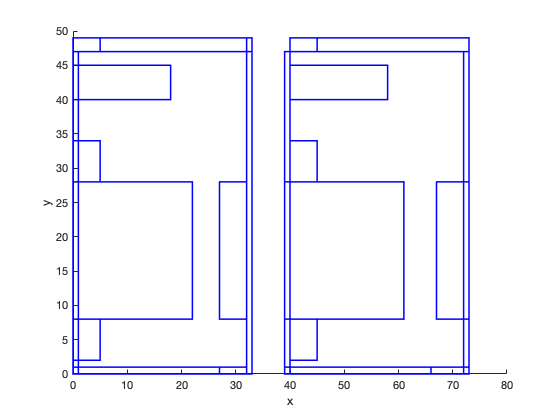
\includegraphics[width=10cm]{figures/test_complex_situation_pic_top.png}
\end{figure}
\begin{figure}[htb]
    \centering
    \caption{常见室内空间处理后建模-侧视图}
    \label{fig:test_common_situation_processed_pic_lean}
    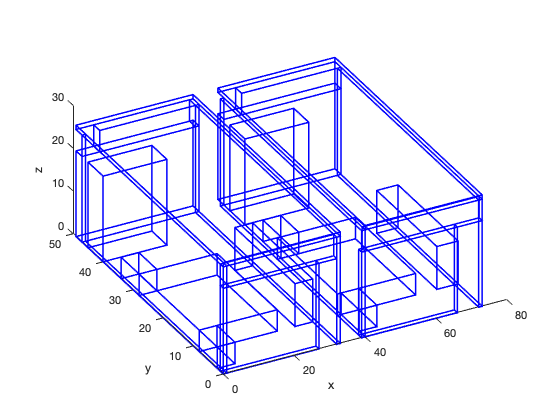
\includegraphics[width=10cm]{figures/test_complex_situation_pic_lean.png}
\end{figure}
\begin{figure}[htb]
    \centering
    \caption{复杂室内空间最短路径结果}
    \label{fig:test_complex_situation_out}
    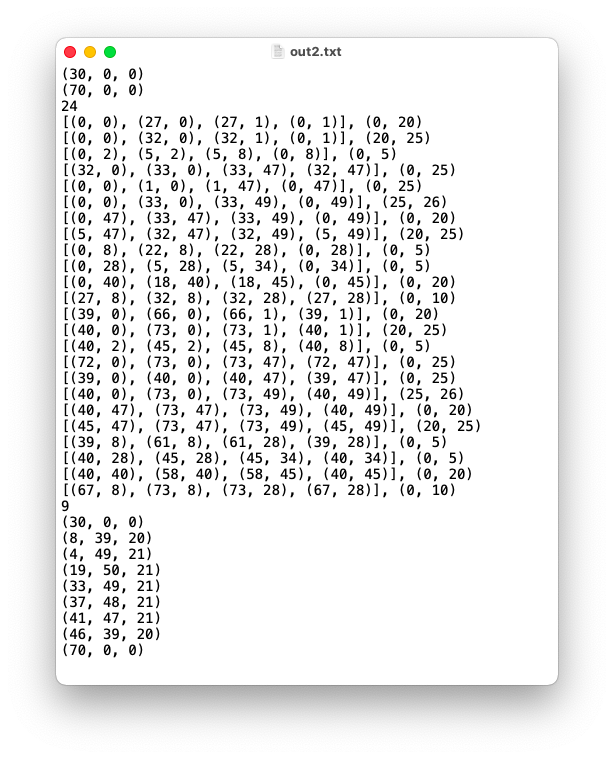
\includegraphics[width=10cm]{figures/test_complex_situation_out.png}
\end{figure}
\begin{figure}[htb]
    \centering
    \caption{复杂室内空间最短路径结果-俯视图}
    \label{fig:test_complex_situation_out_top}
    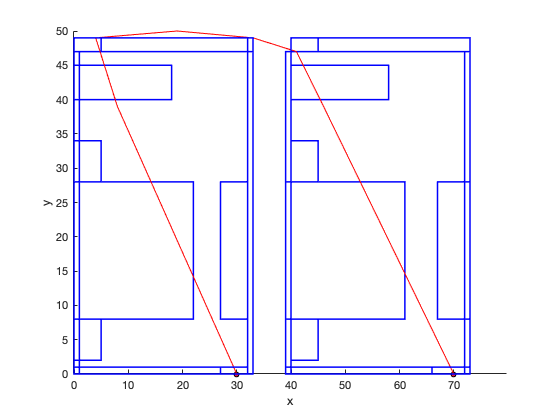
\includegraphics[width=10cm]{figures/test_complex_situation_out_top.png}
\end{figure}
\begin{figure}[htb]
    \centering
    \caption{复杂室内空间最短路径结果-侧视图}
    \label{fig:test_complex_situation_out_lean}
    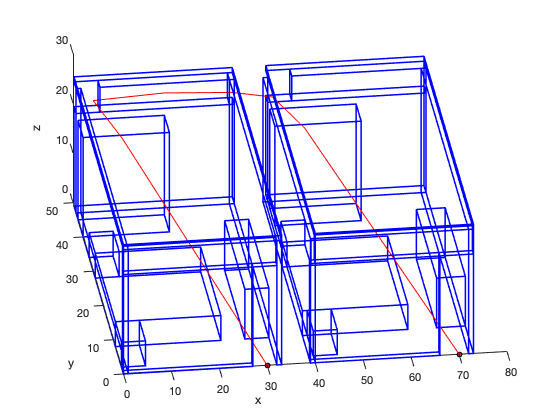
\includegraphics[width=10cm]{figures/test_complex_situation_out_lean.png}
\end{figure}

\subsection{无法到达情况}
\par 除了考虑常见的室内场景和复杂的室内场景,还需要检查算法是否能在无法到达的情况下给出无法找到路径的提示,因此在简单室内场景中将起点和终点分别置于室内和室外,并且房屋密闭不留出门窗,此时是不存在有效路径可以完成起点到终点的。
因此数据如表\ref{tab:test_cant_situation_data},数据包含10个障碍物构成的房屋场景,以及指定精度为0.1。对数据进行离散到精度0.1的操作,得到的数据为表\ref{tab:test_not_situation_processed_data},此时将处理后的障碍物数据绘制到Matlab中,可以得到的建模信息的俯视图和侧视图分别为图\ref{fig:test_not_situation_pic_top}和图\ref{fig:test_not_situation_pic_lean}。
此时使用算法求解起点(2, 1, 0),离散后为(20, 10, 0),到终点(0.1, 5, 0.1),离散后为(1, 50, 1)的最短路径,此时算法输出为图\ref{fig:test_not_situation_out},无路径信息表示未找到有效路径,符合我们设计的条件。
\begin{table}[htb]
    \centering
    \caption{无法到达情况空间测试数据}
    \label{tab:test_cant_situation_data}
    \begin{tabular}{cccc}
        \toprule
        起点&终点&障碍物&精度\\
        \midrule
        \multirow{10}*{(2, 1, 0)}&\multirow{10}*{(0.1, 5, 0.1)}&(0.25, 0.3), (0.25, 0.8), 0.5, [0, 0.5]&\multirow{10}*{0.1}\\
        ~&~&(1.1, 0.8), (1.1, 2.9), 2.2, [0, 0.5]&~\\
        ~&~&(0.25, 2.9), (0.25, 3.4), 0.5, [0, 0.5]&~\\
        ~&~&(0.9, 4), (0.9, 4.5), 1.8, [0, 2]&~\\
        ~&~&(3, 0.8), (3, 2.9), 0.6, [0, 1]&~\\
        ~&~&(1.7, 0), (1.7, 0.1), 3.3, [0, 2.5]&~\\
        ~&~&(1.7, 4.7), (1.7, 4.8), 3.3, [0, 2.5]&~\\
        ~&~&(0.05, 0), (0.05, 4.8), 0.1, [0, 2.5]&~\\
        ~&~&(3.35, 0), (3.35, 4.8), 0.1, [0, 2.5]&~\\
        ~&~&(1.7, 0), (1.7, 4.8), 3.3, [2.5, 2.6]&~\\
        \bottomrule
    \end{tabular}
\end{table}
\begin{table}[htb]
    \centering
    \caption{无法到达情况空间处理后数据}
    \label{tab:test_not_situation_processed_data}
    \begin{tabular}{ccc}
        \toprule
        起点&终点&障碍物\\
        \midrule
        \multirow{10}*{(20, 0, 0)}&\multirow{10}*{(1, 50, 1)}&(0, 2), (5, 2), (5, 8), (0, 8), [0, 5]\\
        ~&~&[(0, 8), (22, 8), (22, 28), (0, 28)], [0, 5]\\
        ~&~&[(0, 28), (5, 28), (5, 34), (0, 34)], [0, 5]\\
        ~&~&[(0, 40), (18, 40), (18, 45), (0, 45)], [0, 20]\\
        ~&~&[(27, 8), (32, 8), (32, 28), (27, 28)], [0, 10]\\
        ~&~&[(0, 0), (33, 0), (33, 1), (0, 1)], [0, 25]\\
        ~&~&[(0, 47), (33, 47), (33, 47), (0, 47)], [0, 25]\\
        ~&~&[(0, 0), (1, 0), (1, 47), (0, 47)], [0, 25]\\
        ~&~&[(33, 0), (34, 0), (34, 47), (33, 47)], [0, 25]\\
        ~&~&[(0, 0), (33, 0), (33, 47), (0, 47)], [25, 26]\\
    \end{tabular}
\end{table}
\begin{figure}[htb]
    \centering
    \caption{无法到达情况空间建模-俯视图}
    \label{fig:test_not_situation_pic_top}
    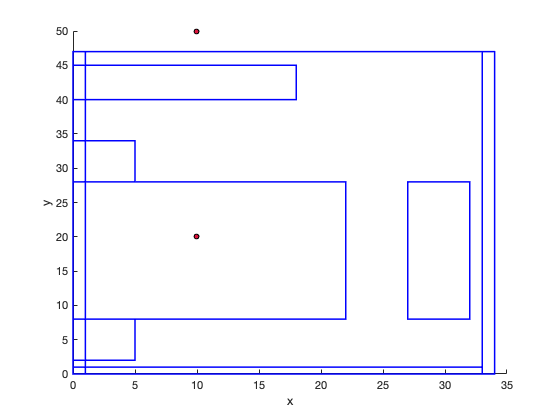
\includegraphics[width=10cm]{figures/test_not_situation_pic_top.png}
\end{figure}
\begin{figure}[htb]
    \centering
    \caption{无法到达情况空间建模-侧视图}
    \label{fig:test_not_situation_pic_lean}
    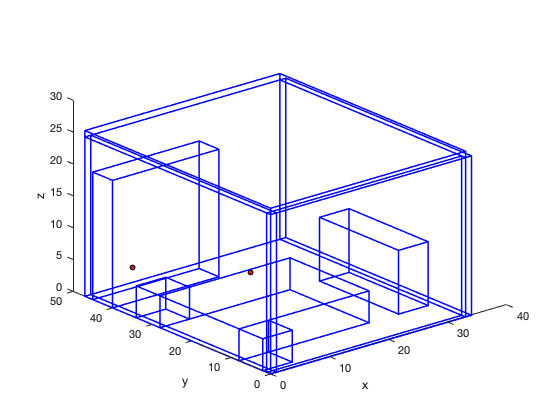
\includegraphics[width=10cm]{figures/test_not_situation_pic_lean.png}
\end{figure}
\begin{figure}[htb]
    \centering
    \caption{无法到达情况算法输出}
    \label{fig:test_not_situation_out}
    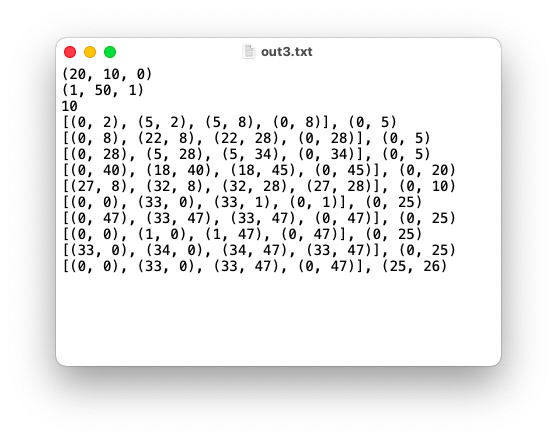
\includegraphics[width=10cm]{figures/test_not_situation_out.png}
\end{figure}

\section{本章总结}
\par{\kaishu 本章主要是对整个算法正确性进行了测试,使用了相关的测试样例和使用了Matlab绘图辅助显示。对主要模块:数据处理算法、路径求解算法进行了测试并分析,数据处理算法主要是代码\ref{code:obstacle_vertice_process}的应用,即将输入只包含底面两中点、边长和z轴范围的障碍物数据处理出底面顶点坐标信息,进而可以被后续算法使用;
路径求解算法主要测试关于使用BFS或A*算法求解起点到终点的格点路径,以及使用公式\ref{con:innerABandCD}和\ref{con:innerDAandBC}的应用以判断线段与障碍物的关系以判断是否路径可以拟合。
\par 其次是对整个算法进行综合测试,构造了常见室内场景空间、复杂场景空间以及无法到达情况空间的数据以测试算法正确性,通过分析算法输出和Matlab辅助显示判断算法是否符合预期效果。
\par 至此,整个算法已经完成构思、编码和测试的环节。}
%%%=== 参考文献 ========%%%
\cleardoublepage\phantomsection
\addcontentsline{toc}{chapter}{参考文献}
\begin{thebibliography}{00}

  \bibitem{r1} 作者. 文章题目 [J].  期刊名, 出版年份,卷号(期数): 起止页码.

  \bibitem{r2} 作者. 书名 [M]. 版次. 出版地:出版单位,出版年份:起止页码.

  \bibitem{r3} 邓建松等, 《\LaTeXe~科技排版指南》, 科学出版社.

  \bibitem{r4} 吴凌云, 《CTeX~FAQ (常见问题集)》, \textit{Version~0.4}, June 21, 2004.

  \bibitem{r5} Herbert Vo\ss, Mathmode, \url{http://www.tex.ac.uk/ctan/info/math/voss/mathmode/Mathmode.pdf}.


\end{thebibliography}

% !Mode:: "TeX:UTF-8"
%%%%%%%%%%%%%%%%%%%%%%%%%%%%-------致谢--------%%%%%%%%%%%%%%%%%%%%%%%%%%%%%%%%

\acknowledgement
\addcontentsline{toc}{chapter}{致谢}


感谢你, 感谢他和她, 感谢大家.











 %%%致谢

\clearpage
\end{document}